\documentclass[tikz,border=5mm]{standalone}
\usepackage{xcolor}

\begin{document}
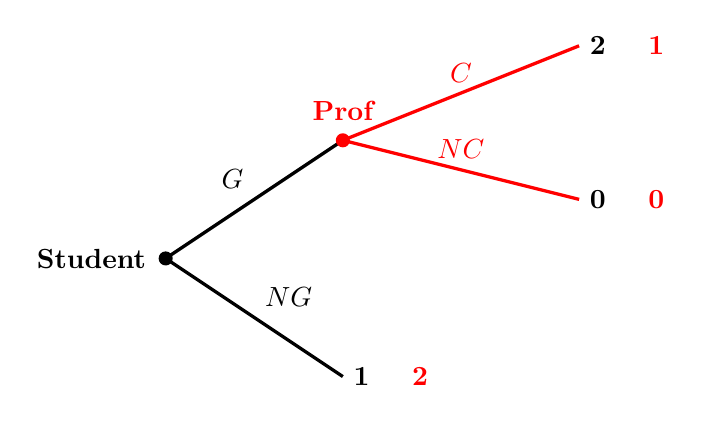
\begin{tikzpicture}[
    scale=1.5,
    font=\bfseries,
    dot/.style={circle, fill=#1, inner sep=1.8pt},
    dot/.default=black,
    line width=1.2pt
]

    % Coordinates
    \coordinate (root) at (0, 0);
    \coordinate (eve_top) at (1.5, 1);
    \coordinate (eve_bot) at (1.5, -1);
    
    \coordinate (leaf1) at (3.5, 1.8);
    \coordinate (leaf2) at (3.5, 0.5);

    % Level 1 branches (Adam)
    \draw[black] (root) -- (eve_top) node[midway, above left] {$G$};
    \draw[black] (root) -- (eve_bot) node[midway, above right] {$NG$};

    % Level 2 branches (Eve)
    \draw[red] (eve_top) -- (leaf1) node[midway, above] {$C$};
    \draw[red] (eve_top) -- (leaf2) node[midway, above] {$NC$};

    % Nodes
    \node[dot=black, label=left:Student] at (root) {};
    \node[dot=red, label={[red]above:Prof}] at (eve_top) {};

    % Payoffs
    \node[right] at (eve_bot) {1 \quad \textcolor{red}{2}};
    \node[right] at (leaf1) {2 \quad \textcolor{red}{1}};
    \node[right] at (leaf2) {0 \quad \textcolor{red}{0}};
    
\end{tikzpicture}
\end{document}